\documentclass{standalone}
\usepackage{tkz-base}
\usepackage{tkz-fct}
\usepackage{tkz-euclide}
\usepackage{tikz}
\begin{document}
    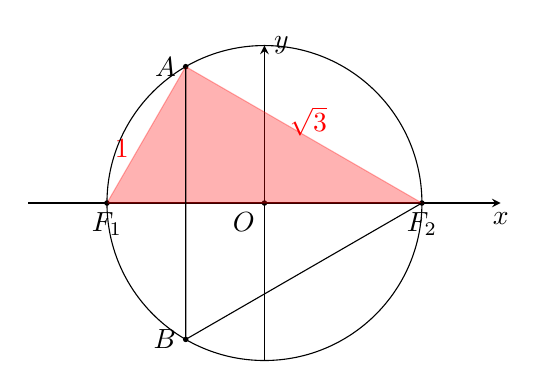
\begin{tikzpicture}
        \pgfmathsetmacro\xx{3}
        \pgfmathsetmacro\y{2}
        \pgfmathsetmacro\a{sqrt(3)-1}
        \pgfmathsetmacro\c{2}
        \pgfmathsetmacro\b{sqrt(abs(\c^2-\a^2))}
        \pgfmathsetmacro\px{-1}
        \pgfmathsetmacro\py{sqrt(-1*\b^2*(1-((\px)^2)/\a^2))}
        \coordinate (O) at (0,0);
        \coordinate (F1) at (-\c,0);
        \coordinate (F2) at (\c,0);
        \coordinate (A) at (\px,\py);
        \coordinate (B) at (\px,-\py);
        \tkzInit[ymax=\y,ymin=-\y,xmax=\xx,xmin=-\xx] 
        \tkzFctPar[samples=400,domain=-0.4*pi:0.4*pi]{\a/(cos(t))}{\b*(tan(t))}
        \tkzFctPar[samples=400,domain=0.6*pi:1.4*pi]{\a/(cos(t))}{\b*(tan(t))}
        \draw[-stealth] (-\xx,0) -- (\xx,0) node [below] {$x$};
        \draw[-stealth] (0,-\y) -- (0,\y) node [right] {$y$};
        \fill (O) node [below left] {$O$} circle (1pt);
        \fill (F1) node [below] {$F_1$} circle (1pt);
        \fill (F2) node [below] {$F_2$} circle (1pt);
        \fill (A) node [left] {$A$} circle (1pt);
        \fill (B) node [left] {$B$} circle (1pt);
        \filldraw[red,opacity = 0.3] (F1) -- (A) node[left,pos=0.4,opacity=1]{$1$}-- (F2)node[right,pos=0.4,opacity=1]{$\sqrt{3}$}-- cycle;
        \draw (A) --(B)--(F2);
        \draw (O) circle (\c);
    
    \end{tikzpicture}
\end{document}